% !TEX encoding = UTF-8 Unicode
\documentclass[12pt,a4paper,english
% ,twoside,openright
]{tunithesis}

\special{papersize=210mm,297mm}

\author{Roosa Kuusivaara \& Väinö-Waltteri Granat}
\title{Signal processing in digital holography - Report} % primary title (for front page)
\thesistype{Laboratory Report} % or Bachelor of Science, Laboratory Report...


\usepackage{lastpage}
\usepackage[english]{babel}
\usepackage[
backend=biber,
style=numeric,
citestyle=numeric,
autocite=inline
]{biblatex}
\usepackage{csquotes}

\addbibresource{references.bib} %Imports bibliography file


\definecolor{tunipurple}{RGB}{78, 0, 142}

\newcommand\todo[1]{{\color{red}!!!TODO: #1}} % Remark text in braces appears in red
\newcommand{\angs}{\textsl{\AA}}              % , e.g. slanted symbol for Ångstöm
% Preparatory content ends here


\pagenumbering{roman} % was: {Roman}
\pagestyle{headings}
\begin{document}

% Special trick so that internal macros (denoted with @ in their name)
% can be used outside the cls file (e.g. \@author)
\makeatletter

% Create the title page.
% First the logo. Check its language.
\thispagestyle{empty}
\vspace*{-.5cm}\noindent

\begin{figure}
    \vspace{-1.3cm}
    \advance\leftskip-2.5cm
    \noindent
\includegraphics{img/tunilogo.png}
\end{figure}
 
\vspace{2.5cm}
\begin{flushright}
\noindent\textsf{\LARGE{\@author}}

\noindent\vspace{0.5cm}

\noindent\Huge{\textsf{\textbf{\textcolor{tunipurple}{\@title}}}}
\end{flushright}
\vspace{13.7cm} % adjust to 12.7 this if thesis title needs two lines

% Last some additional info to the bottom-right corner
\begin{flushright}  
    \begin{spacing}{1.0}
      \textsf{Faculty of Information Technology and Communication Sciences (ITC)\\
      \@thesistype\\}
    \end{spacing}
\end{flushright}

% Leave the backside of title page empty in twoside mode
\if@twoside
\clearpage
\fi

% Turn off page numbering for the first pages
\pagenumbering{gobble}


% Some fields in abstract are automated, namely those with \@ (author,
% title, thesis type).
\chapter*{Abstract}
\begin{spacing}{1.0}
\noindent \@author: \@title\\
\@thesistype\\
Tampere University\\
Master’s Degree Programme in Signal Processing\\
November 2023 \\
\end{spacing}
\noindent\rule{12cm}{0.4pt}

\vspace{0.5cm}

% ---------------------------------------
% Abstract and keywords
% ---------------------------------------

\noindent
This report documents the work done in the Signal processing in digital holography assingment as a part of the Advanced signal processing laboratory course. In this assignment we familiazired ourselves with basics of intereference based holography.
~

\noindent\textbf{Keywords:} M.Sc. thesis, layout, writing style.

~

\noindent The originality of this thesis has been checked using the Turnitin Originality Check service.


% Add the table of contents


\setcounter{tocdepth}{3}              % How many header level are included
\tableofcontents                      % Create TOC


% The actual text begins here and page numbering changes to 1,2...
% Leave the backside of title empty in twoside mode
\if@twoside
%\newpage
\cleardoublepage
\fi


\renewcommand{\chaptername}{} % This disables the prefix 'Chapter' or
                              % 'Luku' in page headers (in 'twoside'
                              % mode)


\chapter{Introduction}
\label{ch:intro}
In this report we describe our work done in the 'Signal processing in digital holography' laboratory assignment for the Advanced Signal Processing Laboratory course. In this assignment we used a Mach-Zehnder interferometer to record holographic images and Matlab to reconstruct the object from the recorded wavefront.

\pagenumbering{arabic}
\setcounter{page}{1} 

\chapter{Methodology}
This section describes the method we used to capture the holograms and reconstruct the objects.
\label{sec:methodology}
\subsection{Experiment setup}
Holographic imagery relies on the phenomena of light wave superpositions. In this assignment the object is captured using a Mach-Zehnder interferometer, where a monochromatic laser is used to produce two wavefronts. The first wavefront passes trough the object which we want to record, and the second wavefront is used as reference wavefront. The wavefront are the combined to a single wavefront via the interference phenomena, so that one of the wavefronts is combined with the other wavefront in a slight angle, causing a phase difference. The resulting total wave is then captured with a CMOS camera to produce a image file. The phase difference is detectable as fringes in the captured images. The complete setup for the experiment is shown in figure~\ref{fig:lab_setup}.

\begin{figure}
  \centering
  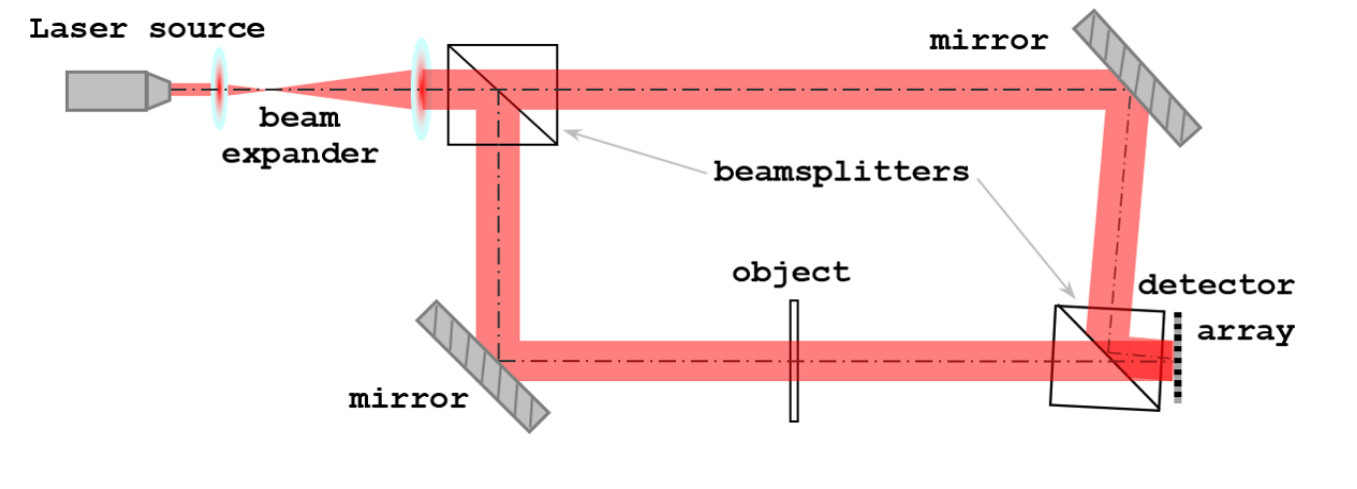
\includegraphics[width=\columnwidth]{img/lab_setup.png}
  \caption{Experiment was done using a Mach-Zehnder interferometer. Taken from~\cite{assignment}}
  \label{fig:lab_setup}
\end{figure}


\subsection{Object reconstruction}
The object can be extracted from the captured hologram, using a two step method.

First step is to use Fourier filtering to extract the object wave. Since we know that the hologram is defined by the following equation:
\begin{equation}
H(x, y) = E_0(x, y)^2 + E_r(x, y)^2 + U_0(x, y)U_r^*(x, y) + U_0^*(x, y)U_r(x, y)
\end{equation}

Where $H(x,y)$ is the hologram wavefront in given position, $E_0$ is the objects amplitude, $E_r$ is the reference wave's amplitude, $U_r$ is the reference wavefront and $U_0$ is the object wavefront which we want to extract.

\begin{equation}
\mathcal{F}[H(x, y)] = \mathcal{F}\left[E_0(x, y)^2 + E_r(x, y)^2\right] + \mathcal{F}\left[U_0(x, y)E_r \exp(i2\pi\eta)\right] + \mathcal{F}\left[U_0^*(x, y)E_r \exp(-i2\pi\eta)\right]
\end{equation}



\chapter{Results}
\label{sec:results}

\chapter{Conclusions}
\label{ch:conclusions}

%
% The bibliography, i.e the list of references
%
\newpage

\printbibliography[title=References]
\addcontentsline{toc}{chapter}{References}

\end{document}

